% Created 2013-12-13 Fri 11:21
\documentclass[11pt]{article}
\usepackage[utf8]{inputenc}
\usepackage[T1]{fontenc}
\usepackage{fixltx2e}
\usepackage{graphicx}
\usepackage{longtable}
\usepackage{float}
\usepackage{wrapfig}
\usepackage{soul}
\usepackage{textcomp}
\usepackage{marvosym}
\usepackage{wasysym}
\usepackage{latexsym}
\usepackage{amssymb}
\usepackage{hyperref}
\tolerance=1000
\providecommand{\alert}[1]{\textbf{#1}}

\title{r2r\_{}vocabs}
\author{Drumbeat}
\date{\today}
\hypersetup{
  pdfkeywords={},
  pdfsubject={},
  pdfcreator={Emacs Org-mode version 7.9.3f}}

\begin{document}

\maketitle

\setcounter{tocdepth}{3}
\tableofcontents
\vspace*{1cm}
\section{Introduction}
\label{sec-1}

This document provides descriptions, policies and scripts used to process vocabulary terms associated with the R2R eventlog project. The source is maintained as an org-mode file, accessed using the emacs environment. The directory containing this file and other files related to it can be found at the \href{https://github.com/amaffei/r2relogvocabs}{GitHub repository}.
\section{R2R Vocabulary Workflow overview}
\label{sec-2}

The R2R Eventlogger is an application that provides oceanographers with a way to record events that happen during a research cruise. This application is base on the \href{https://midas.psi.ch/elog/}{ELOG Weblog} open source package. The R2R project has modified this software so that controlled vocabularies can be used to configure participants, instruments, intstrument actions, and organizations at the start of a cruise.

In addition to making use of a given set of controlled vocabulary terms, oceanographers are allowed to create and insert new terms, specific to their own research needs. It is up to the R2R project whether or not to add these to it's own controlled vocabularies or oceanographic community vocabularies.

The preferred oceanographic community vocabularies are served as a service of the \href{http://www.bodc.ac.uk/products/web_services/vocab/}{NERC Vocabulary Server (NVS)}, that is supported and maintained by the \href{http://www.bodc.ac.uk/}{British Oceanographic Data Centre}. 

The workflow described here only handles instrument and instrument action vocabulary terms.
\subsection{Workflow diagram}
\label{sec-2-1}

The following is a diagram shows how configuration files, returned from past oceanographic research cruises, are processed by the R2R project. The goal of this project is to provide the following outputs:
\begin{itemize}
\item an updated list of controlled vocabulary terms to be integrated into future releases of the R2R Eventlogger webapp.
\item a list of new/modified controlled vocabulary terms to be submitted to the NVS governance process so that the pertinent vocabularies served by NVS can be updated for use by the larger oceanographic community
\end{itemize}
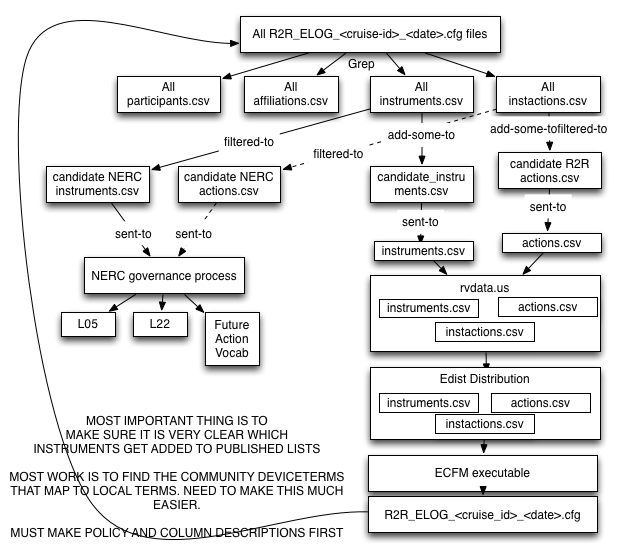
\includegraphics[width=.9\linewidth]{//inst_vocab_wflow.png}
\section{Description of R2R Eventlogger application related files}
\label{sec-3}

The followig CSV files are included in the R2R Edist software distribution. This software distribution includes the R2R Evenlogger application in addition to the environment (auxillary files, etc.) required to run it.
\subsection{<cruise-id>/}
\label{sec-3-1}
\subsection{<cruise-id>/}
\label{sec-3-2}
\section{}

\end{document}
